\documentclass[]{acmsiggraph}
\usepackage{algorithm}
\usepackage[noend]{algpseudocode}
\TOGonlineid{45678}
\TOGvolume{0}
\TOGnumber{0}
\TOGarticleDOI{0}
\TOGprojectURL{}
\TOGvideoURL{}
\TOGdataURL{}
\TOGcodeURL{}
\usepackage{color}
%\definecolor{red}{rgb}{0.9, 0.17, 0.31}
\usepackage{multirow}
\usepackage{subfig}
\usepackage{xcolor}
\usepackage{lipsum}
\usepackage{listings}
\usepackage{graphicx}
\usepackage{glsllst} 
\usepackage{rmlst}  
\usepackage{amsmath}
\usepackage{hyperref}
\usepackage[english]{babel}
\usepackage[square,numbers]{natbib}
\usepackage{graphicx}
\usepackage{subcaption}
\bibliographystyle{abbrvnat}
\lstset{
	backgroundcolor=\color[rgb]{0.95, 0.95, 0.95},
	tabsize=3,
	%rulecolor=,
	basicstyle=\footnotesize\ttfamily,
	upquote=true,
	aboveskip={1.5\baselineskip},
	columns=fixed,
	showstringspaces=false,
	extendedchars=true,
	breaklines=true,
	prebreak = \raisebox{0ex}[0ex][0ex]{\ensuremath{\hookleftarrow}},
	frame=none,
	aboveskip=15pt,
	belowskip=8pt,
	captionpos=t,
	showtabs=false,
	showspaces=false,
	showstringspaces=false,
	identifierstyle=\ttfamily,
	%keywordstyle=\color{red}\bfseries,
	%keywordstyle=[1]\bfseries\color{syntaxBlue},
	%keywordstyle=[2]\bfseries\color{syntaxRed},
	%keywordstyle=[3]\color{blue}\bfseries,
	%keywordstyle=[4]\bfseries\color{syntaxBlue},
	commentstyle=\color[rgb]{0.082,0.639,0.082},
	keywordstyle=[1]\bfseries\color[rgb]{0,0,0.75},
	keywordstyle=[2]\bfseries\color[rgb]{0.5,0.0,0.0},
	keywordstyle=[3]\bfseries\color[rgb]{0.127,0.427,0.514},
	keywordstyle=[4]\bfseries\color[rgb]{0.4,0.4,0.4},
	stringstyle=\color[rgb]{0.639,0.082,0.082},
}

\title{Lung Covid Infection Segmentation Using U-Net Deep Learning Model}

\author{Anh Quan Nguyen BI12-365\thanks{e-mail: quanna.bi12-365@st.usth.edu.vn}\\University of Science and Technology of Hanoi}
\pdfauthor{Anh Quan Nguyen}

\keywords{rendering}

\begin{document}

\maketitle


\begin{abstract}
This study investigates the application of a U-Net deep learning model for segmenting lung regions infected with COVID-19 in X-ray images. We emphasize the importance of accurate segmentation in effectively diagnosing and analyzing COVID-19 cases. The U-Net architecture's capability to capture precise spatial information within lung X-rays is highlighted, enabling the model to isolate and delineate COVID-19-infected areas. This segmentation facilitates improved diagnostic accuracy by allowing radiologists to focus on the critical infected regions. Additionally, the segmented data can be utilized to train and enhance computer-aided analysis (CAD) systems, potentially leading to faster and more accurate diagnoses of COVID-19 infections. Overall, this study explores the potential of the U-Net deep learning model for precise segmentation of lung COVID-19 infections in X-ray images, aiming to contribute to more efficient and effective COVID-19 diagnosis.
\end{abstract}
%\keywordlist
%\TOGlinkslist

\section{Introduction}

\subsection{Context and Motivation}
Chest X-rays (CXRs) have become a cornerstone of COVID-19 diagnosis due to their affordability, speed, and widespread availability. However, accurately identifying and segmenting the lung regions infected by the virus remains challenging.  Ground-glass opacities, a hallmark of COVID-19 pneumonia, can be subtle and visually similar to healthy lung tissue. Additionally, radiologists face immense pressure during pandemics.  Therefore, this research is motivated by the development of a computer-aided diagnostic tool for segmenting infected areas in chest X-rays. This approach has the potential to improve diagnostic efficiency and accuracy, alleviate pressure on healthcare systems, and ultimately contribute to a more effective fight against COVID-19.

\subsection{Objectives}
The primary objective of this study is to utilize the application of the deep learning model, specifically the U-Net, in automatically segmenting the infectious area in the lung of the patient through CXRs. Through this exploration, we aim to explore and imply a modern solution to COVID-19 disease diagnosis.

\subsection{Related Works}
Prior research has significantly shaped the landscape of CXRs COVID-19 infection segmentation. Notably, Walid Al-Zyoud et al. \cite{walid2023} implemented various image processing and image analysis techniques to classify the pixels of the background and the infectious areas. Additionally, Anas M. Tahir et al. made noteworthy contributions in localizing and segmenting the infection inside the lung \cite{anas2021}. These influential works not only inform our study but also highlight the evolving nature of X-ray image segmentation, guiding our research within this dynamic field.

\section{Dataset Understanding}
The dataset utilized in this study is a minor part of the COVID-QU-Ex Dataset\cite{chowhury2020}, \cite{degerli2021}, \cite{rahman2021}, \cite{anas2021}. The utilized data are the 11,956 COVID-positive chest X-ray samples, which are separated into 1864 for the training set, 466 for the validation set, and a collection of 583 for the test set. 

Each X-ray image is paired with a corresponding mask image with a resolution of 256x256. The masks are grayscale, with white pixels indicating infectious areas and black pixels representing the non-infection regions.

\begin{figure}[h]\centering
 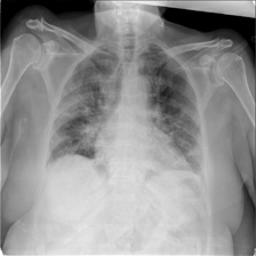
\includegraphics[width=0.75\linewidth]{images/covid_1.png}
 \caption{\label{fig:reference}Sample of chest X-ray image.}
\end{figure}

\begin{figure}[h]\centering
 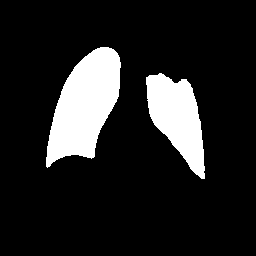
\includegraphics[width=0.75\linewidth]{images/covid_1_mask.png}
 \caption{\label{fig:reference}Corresponding mask.}
\end{figure}

\section{Method}
\subsection{Data Preprocessing}
\paragraph{Min-Max Scaling:}
The images undergo Min-Max scaling operation to ensure consistent pixel value ranges across different images. First, the image is flattened into a 1-D array of pixel values. Then we use the Min-Max scaling formula to scale the pixel values:
\[
X' = \frac{X - X_{\text{min}}}{X_{\text{max}} - X_{\text{min}}}
\]
After that, the array is scaled back into the shape of the image for further image processing and analyzing methods.

This step is crucial for creating a standardized input that facilitates effective model training. Normalization brings pixel values within a standardized range, typically between 0 and 1.

\paragraph{Transfer Learning Preprocessing:}
As transfer learning plays a pivotal role in this approach, the Transfer Learning Preprocessing phase takes center stage, strategically aligning the input data with the nuanced expectations of the pre-trained ResNet34 backbone. In leveraging the profound knowledge encapsulated within ResNet34, acquired during its training on diverse datasets, the process commences with the meticulous application of mean subtraction:
\[ X' = X - \text{Mean} \]
This operation involves subtracting the mean pixel value from each pixel across the entire dataset, effectively centering the input data around zero. Concurrently, channel-wise normalization is employed, systematically scaling pixel values to ensure uniformity and alignment with the model's prescribed input distribution:
\[ X' = \frac{X - \text{Mean pixel value of the specific channel}}{\text{Standard deviation of the channel}} \]
This normalization procedure extends beyond mean subtraction, incorporating channel-wise scaling to harmonize the pixel value distributions with the statistical norms established during the model's original training. Simultaneously, adjustments to the input size are made, conforming to the stipulated dimensions of ResNet34, thereby facilitating a seamless transfer of knowledge. In this experiment, \(256 \times 256 \times 3\) (height $\times$ width $\times$ channel) is selected to fit the input of the model and enhance computational efficiency and training speed.

\paragraph{One-hot Encoding:}
In this method, the original mask from the training set, representing infection and non-infection labels, transforms into a one-hot encoded format. This involves creating a binary matrix with two channels, corresponding to the distinct classes—infectious and non-infection areas. The one-hot encoding serves to convert categorical information into a more structured representation, allowing the neural network to comprehend and learn from the pixel-wise labels effectively. This binary matrix facilitates a clearer delineation between infectious and normal classes during model training, contributing to the accurate segmentation in X-ray imagery. After this process, the mask has the shape of \(256 \times 256 \times 2\) (height $\times$ width $\times$ number of binary maps).

\paragraph{Data Augmentation:}
Data augmentation is introduced to diversify the training dataset, promoting consistency and generalization of the trained model. Horizontal and vertical flips, along with reflective filling, are applied to both input images and their corresponding masks. These augmentations introduce variations in the dataset, reducing the risk of overfitting and enhancing the model's ability to handle diverse patient laying position scenarios. We performed this technique for both training images and the corresponding masks.

\subsection{Model Architecture}
In this research, we applied transfer learning techniques using a U-net Model with ResNet34 encoding backbones. As mentioned above, the model has an input size of 256 x 256 x3 and an output shape of 256 x 256 x 2, the same shape as the one-hot encoded masks. The model includes 24438949 trainable parameters, and ImageNet encoder weights to improve the performance of the training process.

\begin{figure}[h]\centering
 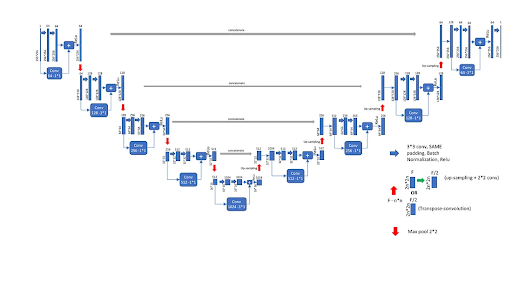
\includegraphics[width=0.75\linewidth]{images/model.png}
 \caption{\label{fig:reference}U-Net with ResNet34 Backbone Architecture.}
\end{figure}

The activation function employed at the final layer is softmax. Softmax activation is pivotal in converting the model's raw output scores into probabilities, ensuring that the sum of probabilities across all classes for each pixel equals 1. This characteristic is essential for the model to produce meaningful and interpretable segmentation results.

\subsection{Evaluation Metrics}
\paragraph{Loss function: Focal Loss + Jaccard Loss}
The Focal Loss is a modification of the standard categorical cross-entropy loss, designed to address class imbalance in segmentation tasks, by reducing the influence of the overwhelmed examples to pay more attention to class with minority examples.
\[ \text{Focal Loss} = -\sum_{i=1}^{n} y_i \cdot \log(p_i) \cdot (1 - p_i)^{\gamma} \]
where $y_i$ represents the true label, $p_i$ represents the predicted probability, and $\gamma$ is a tunable focusing parameter.

The Jaccard Loss, also known as Intersection over Union (IoU) loss or Jaccard Index loss, is a metric commonly used in segmentation tasks to measure the similarity between predicted and ground truth masks. It quantifies the spatial overlap between the two masks, providing a comprehensive assessment of segmentation accuracy.
\[ \text{Jaccard Loss} = 1 - \frac{|A \cap B|}{|A \cup B|} \]

Combining Categorical Focal Loss and Jaccard Loss provides a comprehensive evaluation framework, addressing both class imbalance challenges and spatial accuracy considerations, ensuring a holistic assessment of the model's segmentation performance.

\paragraph{Metric: Intersection Over Union (IoU) score}
The Intersection over Union (IoU) score, also known as the Jaccard Index, quantifies the spatial overlap between predicted and ground truth segmentation masks, offering a concise metric to assess the accuracy of infection localization in X-ray imagery. A higher IoU score indicates better alignment, capturing the model's effectiveness in precisely highlighting the infectious field within the images.
\[ \text{IoU} = \frac{|A \cap B|}{|A \cup B|} \]
where $A$ represents the predicted mask and $B$ represents the ground truth mask.

\paragraph{Optimizer: Adam}
Adam, short for Adaptive Moment Estimation, is an optimization algorithm commonly used in training neural networks; it combines the benefits of both momentum and RMSprop, dynamically adjusting learning rates for each parameter to enhance convergence speed and stability. By maintaining per-parameter learning rates and exponentially decaying averages of past gradients, Adam efficiently navigates complex optimization landscapes, making it a popular choice for deep learning tasks. The learning rate chosen in the operation is 0.001.

\section{Results} \label{sec:overview}
We performed model training for 50 epochs due to the lack of computational and time resources, with 32 images and masks per batch. The predicted result is quite impressive as the value of Loss and IoU score are nearly optimized at the end of the training process.

\begin{figure}[h]\centering
 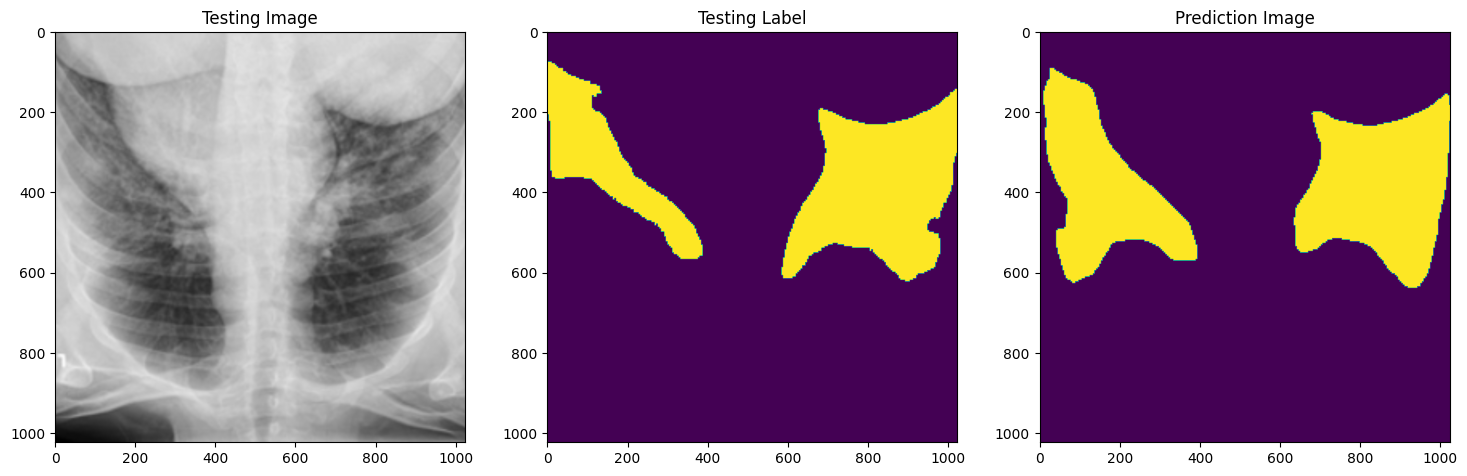
\includegraphics[width=0.75\linewidth]{images/results.png}
 \caption{\label{fig:reference}Visualisation of Original image, original mask, and the predicted mask .}
\end{figure}

\subsection{Loss Function}
The Validation Loss drops significantly from 0.7 to nearly 0.3, and this value seems to be close to the training loss during the last epochs, indicating that the model learned effectively from the training set and can generalize well from the unseen data. 

\begin{figure}[h]\centering
 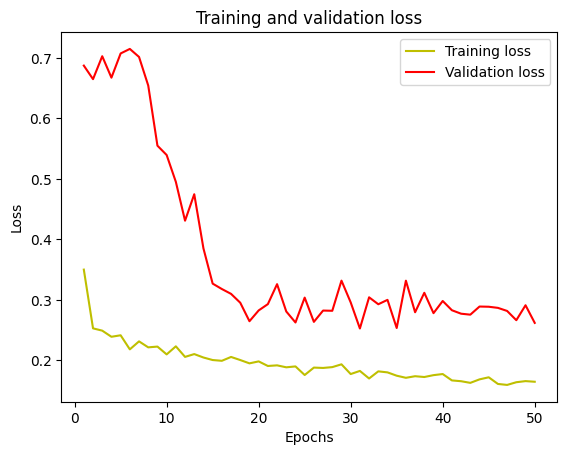
\includegraphics[width=0.75\linewidth]{images/loss.png}
 \caption{\label{fig:reference}Loss function during training.}
\end{figure}

\subsection{IoU Score}
Positive results are also seen in the IoU score chart, where the highest values for training and validation are 0.83 and 0.77, respectively. The small difference between these metrics during training indicates the model's ability to perform consistently well on both seen and unseen data.

\begin{figure}[h]\centering
 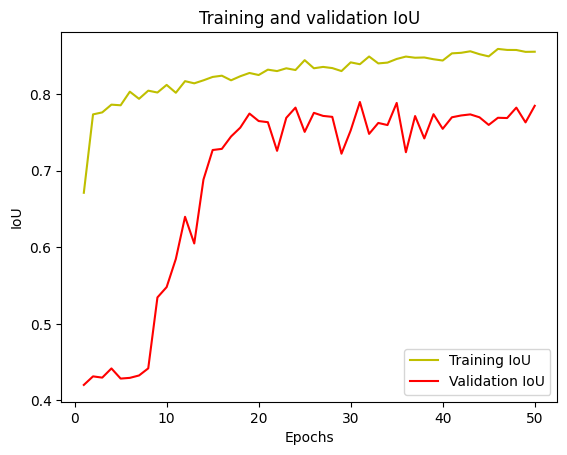
\includegraphics[width=0.75\linewidth]{images/iou.png}
 \caption{\label{fig:reference}IoU Score during training.}
\end{figure}
\section{Discussion}

\subsection{Drawbacks}

\paragraph{Computational Complexity:}The computational demands of Deep Learning model can be significant, posing challenges in resource-constrained environments.

\paragraph{Data Limitation:}The data we experimented with in this research is only a subset of the whole original data and this limited dataset may affect the performance of the methods and model. 

\paragraph{Data Annotation:}Some annotations provided by the authors may not be precise so some areas that the model can perform well may not be noted or be downgraded by the evaluation metrics.

\subsection{Future Works}

\paragraph{Experiment on a more diverse dataset:}Perform training with the rest of the dataset which contains Non-Covid samples to enhance the model operations.

\paragraph{Proper Annotation:}Generate a more accurate set of data annotations that cover most of the infectious areas to boost the evaluation correctness.

\paragraph{Transfer Learning:} Approach this problem with different models and transfer learning backbone to find the most fit methodology.

\paragraph{Real-world Deployment:} Focus on practical aspects of deploying these models in real-world healthcare settings, considering integration with existing systems, scalability, and regulatory compliance for successful deployment.


\bibliography{references}

\end{document}